\documentclass[handout]{beamer}  

%Smaller gap at between top and bottom of block when there are displayed equations
\addtobeamertemplate{block begin}{\setlength\abovedisplayskip{0pt}}
{\setlength{\belowdisplayskip}{0pt}}


\usepackage{setspace}
\linespread{1.3}
\usepackage{amssymb, amsmath, amsthm} 
\usepackage{rotating}
\usepackage{multirow}
\usepackage{graphicx}
\usepackage{synttree}
\usepackage{verbatim}
\usepackage{fancybox}
\usepackage{color}
\usepackage{tikz}
\usetikzlibrary{shapes,backgrounds}
\usepackage{hyperref}
\usetikzlibrary{trees}
\newcommand{\p}{\mathbb{P}}
\newcommand{\expect}{\mathbb{E}}


%\setbeamertemplate{blocks}[rounded][shadow=true] 
%gets rid of bottom navigation bars
\setbeamertemplate{footline}{
   \begin{beamercolorbox}[ht=4ex,leftskip=0.3cm,rightskip=0.3cm]{author in head/foot}
%    \usebeamercolor{UniBlue}
    \vspace{0.1cm}
    %\insertshorttitle \ - \insertdate 
    \hfill \insertframenumber / \inserttotalframenumber
   \end{beamercolorbox}
   \vspace*{0.1cm}
} 


%gets rid of navigation symbols
\setbeamertemplate{navigation symbols}{}


%Include or exclude the notes?
%\setbeameroption{show notes}
\setbeameroption{hide notes}

\title[Econ 103]{Economics 103 -- Statistics for Economists} 
\author[F. DiTraglia]{Francis J.\ DiTraglia}
\institute{University of Pennsylvania}
\date{Lecture 11}
\begin{document} 
%%%%%%%%%%%%%%%%%%%%%%%%%%%%%%%%%%%%%%%%

\begin{frame}[plain]
	\titlepage 
	

\end{frame} 

%%%%%%%%%%%%%%%%%%%%%%%%%%%%%%%%%%%%%%%%


\begin{frame}
\frametitle{Today}

\begin{enumerate}
	\item Discrete RVs -- Part IV
	\item Continuous RVs -- Part I
\end{enumerate}

\end{frame}


%%%%%%%%%%%%%%%%%%%%%%%%%%%%%%%%%%%%%%%%
\begin{frame}
\frametitle{Recall from Last Time:}
\Large
		$$\boxed{E[g(X,Y)] = \sum_x\sum_y g(x,y)p_{XY}(x,y)}$$
\end{frame}
%%%%%%%%%%%%%%%%%%%%%%%%%%%%%%%%%%%%%%%%


\begin{frame}
\frametitle{Linearity of Expectation, Again}
\framesubtitle{Holds for Continuous RVs as well, but different proof.}
In general, $E[g(X,Y)]\neq g(E[X],E[Y])$. The key exception is when $g$ is a linear function:

\Large
$$\boxed{E[aX + bY + c] = aE[X] + bE[Y] + c}$$

\normalsize
where $X,Y$ are random variables and $a,b,c$ are constants.
\end{frame}
%%%%%%%%%%%%%%%%%%%%%%%%%%%%%%%%%%%%%%%%
\begin{frame}
\frametitle{Proof of Linearity of Expectation for Discrete RVs}
\footnotesize
\begin{eqnarray*}
	E[aX+bY+c] &=& \sum_x \sum_y (ax+by+c) p(x,y) \\
		&=& \pause \sum_x \sum_y\left[ axp(x,y) + byp(x,y) + cp(x,y)\right]\\
		&=&\pause \alert{a} \sum_x \sum_y xp(x,y) + \alert{b}\sum_y \sum_x y p(x,y) + \alert{c} \sum_y \sum_x  p(x,y) \\
		&=& \pause a \sum_x \sum_y xp(x,y) + b\sum_y \sum_x y p(x,y) + \alert{c}\\
				&=& \pause a \sum_{\alert{x}} \alert{x} \left(\sum_{\alert{y}} p(x,y)\right) + b\sum_{\alert{y}} \alert{y} \left(\sum_{\alert{x}}  p(x,y)\right) + c\\
		&=& \pause a\sum_x x \alert{p(x)} + b\sum_y y  \alert{p(y)}+c\\
		&=& \pause aE[X] + bE[Y] + c
\end{eqnarray*}
\end{frame}

%%%%%%%%%%%%%%%%%%%%%%%%%%%%%%%%%%%%%%%%

\begin{frame}
\frametitle{Application: Shortcut Formula for Variance}

By the Linearity of Expectation, 
\begin{eqnarray*}
	Var(X) &=&  E[(X - \mu)^2] = \pause E[X^2 - 2\mu X + \mu^2]\\
		&=& \pause E[X^2] - 2\mu E[X] + \mu^2\\
		&=& \pause E[X^2] - 2\mu^2 + \mu^2\\
		&=& \pause E[X^2] - \mu^2
\end{eqnarray*}

\alert{We saw in a previous lecture that it's typically much easier to calculate variances using the shortcut formula.}

\end{frame}

%%%%%%%%%%%%%%%%%%%%%%%%%%%%%%%%%%%%%%%%

\begin{frame}
\frametitle{Another Application: Shortcut Formula for Covariance}
\alert{Similar to Shortcut for Variance: in fact $Var(X) = Cov(X,X)$}
\begin{eqnarray*}
	Cov(X,Y)&=& E[(X - \mu_X)(Y-\mu_Y)]\\
			&=& E[XY - \mu_X Y - \mu_Y X + \mu_X \mu_Y]\\
			&\vdots& \\
			%&=&E[XY] - \mu_xE[Y] - \mu_Y E[X] + \mu_X \mu_Y\\
			%&=& E[XY] - \mu_X\mu_Y - \mu_Y\mu_X + \mu_X \mu_Y\\
			%&=& E[XY] - \mu_X \mu_Y\\
			&=& E[XY] - E[X]E[Y]
\end{eqnarray*}

\hfill \alert{You'll fill in the details for homework...}
\end{frame}


%%%%%%%%%%%%%%%%%%%%%%%%%%%%%%%%%%%%%%%%
\begin{frame}
\frametitle{Expected Value of Sum = Sum of Expected Values}
Repeatedly applying the linearity of expectation,
$$E[X_1 + X_2 + \hdots + X_n] = E[X_1] + E[X_2] + \hdots + E[X_n]$$
regardless of how the RVs $X_1, \hdots, X_n$ are related to each other. In particular it \alert{doesn't matter if they're dependent or independent}.


\end{frame}
%%%%%%%%%%%%%%%%%%%%%%%%%%%%%%%%%%%%%%%%
\begin{frame}
\frametitle{Independent and Identically Distributed (iid) RVs}

\begin{block}{Example}
	$X_1, X_2, \hdots X_n \sim \mbox{iid Bernoulli}(p)$
\end{block}

\begin{block}{Independent}
Joint pmf equals product of marginal pmfs (see last lecture): Knowing the realization of one of the RVs gives no information about the others.
\end{block}

\begin{block}{Identically Distributed}
Each $X_i$ is the same kind of RV, with the same values for any parameters. (Hence same pmf, cdf, mean, variance, etc.)
\end{block}

\end{frame}
%%%%%%%%%%%%%%%%%%%%%%%%%%%%%%%%%%%%%%%%
\begin{frame}
\frametitle{Binomial$(n,p)$ Random Variable}

\begin{block}{Definition}
Sum of $n$ independent Bernoulli RVs, each with probability of ``success,'' i.e.\ 1, equal to $p$
\end{block}


\begin{block}{Parameters}
$p =$ probability of ``success,'' $n=$ \# of trials
\end{block}


\begin{block}{Support} 
$\{0, 1, 2, \hdots, n\}$
\end{block}


\begin{alertblock}{Using Our New Notation}
Let $X_1, X_2, \hdots, X_n \sim \mbox{iid Bernoulli}(p)$, $Y = X_1 + X_2 + \hdots + X_n$. Then $Y \sim \mbox{Binomial}(n,p)$.
\end{alertblock}


\end{frame}
%%%%%%%%%%%%%%%%%%%%%%%%%%%%%%%%%%%%%%%%
\begin{frame}
\frametitle{Which of these is the PMF of a Binomial$(n,p)$ RV? \hfill 
\includegraphics[scale = 0.05]{./images/clicker}}

\begin{enumerate}[(a)]
	\item $p(x) = p^x (1-p)^{n-x}$
	\item $p(x) = {n \choose x} p^x (1-p)^{n-x}$
	\item $p(x) = {x \choose n} p^x$
	\item $p(x) = {n \choose x} p^{n-x} (1-p)^{x}$
	\item $p(x) = p^n (1-p)^{x}$
\end{enumerate}

\pause
 
$$\alert{p(x) = {n \choose x} p^x (1-p)^{n-x}}$$ 



\end{frame}
%%%%%%%%%%%%%%%%%%%%%%%%%%%%%%%%%%%%%%%%
\begin{frame}
\frametitle{Expected Value of Binomial RV}

Use the fact that a Binomial$(n,p)$ RV is defined as the sum of $n$ iid Bernoulli$(p)$ Random Variables and the Linearity of Expectation:
\begin{eqnarray*}
E[Y] &=& E[X_1 + X_2 + \hdots + X_n] = \pause E[X_1] + E[X_2] + \hdots +E[X_n]\\
	&=&\pause p + p + \hdots + p\\
	&=& \pause \alert{np}
\end{eqnarray*}
\vspace{3em}
\end{frame}

%%%%%%%%%%%%%%%%%%%%%%%%%%%%%%%%%%%%%%%%
\begin{frame}
\huge
Extremely Important:\\
\vspace{1em}
\alert{Variance of Sum $\neq$ Sum of Variances!}
\end{frame}
%%%%%%%%%%%%%%%%%%%%%%%%%%%%%%%%%%%%%%%%
\begin{frame}
\frametitle{Variance of a Sum}
\footnotesize
\begin{eqnarray*}
	Var(aX + bY) &=& E\left[\left\{\left( aX + bY\right) - E[aX + bY]\right\}^2  \right]\\ \pause
	&=& E\left[  \left\{a (X - \mu_X) + b(Y - \mu_Y)\right\}^2 \right]\\ \pause
	&=& E\left[a^2(X-\mu_X)^2 + b^2(Y-\mu_Y)^2 + 2ab(X-\mu_X)(Y-\mu_Y)  \right]\\ \pause
	&=&a^2E[(X-\mu_X)^2] + b^2 E[(Y-\mu_Y)^2] + 2ab E[(X-\mu_X)(Y-\mu_Y)]\\ \pause
	&=& \alert{a^2 Var(X) + b^2 Var(Y) + 2ab Cov(X,Y)}
\end{eqnarray*}


\vspace{3em}
\normalsize
Since $\sigma_{XY} = \rho\sigma_X \sigma_Y$, this is sometimes written as:
$$\alert{\boxed{Var(aX + bY) = a^2 \sigma_X^2 + b^2 \sigma_Y^2 + 2ab \rho \sigma_X \sigma_Y}}$$
\end{frame}
%%%%%%%%%%%%%%%%%%%%%%%%%%%%%%%%%%%%%%%%
\begin{frame}
\frametitle{Independence $\Rightarrow Var(X+Y) = Var(X) + Var(Y)$}

We showed last time that if $X$ and $Y$ are independent, $Cov(X,Y)=0$. Hence, independence implies
\begin{eqnarray*}
	Var(X + Y) &=& Var(X) + Var(Y) + 2 Cov(X,Y)\\
			&=& \alert{Var(X) +Var(Y)}
\end{eqnarray*}


\begin{block}{This is also true for more than two RVs}
If $X_1, X_2, \hdots, X_n$ are independent, then
	$$Var(X_1 + X_2 + \hdots X_n) = Var(X_1) + Var(X_2) + \hdots + Var(X_n)$$
\end{block}

\end{frame}
%%%%%%%%%%%%%%%%%%%%%%%%%%%%%%%%%%%%%%%%
\begin{frame}
\frametitle{Crucial Distinction}
\begin{block}{Expected Value}
It is \alert{always} true that
	$$E[X_1 + X_2 + \hdots + X_n] = E[X_1] + E[X_2] + \hdots + E[X_n]$$
\end{block}


\begin{block}{Variance}
It is \alert{not true in general} that 
	$$Var[X_1 + X_2 + \hdots + X_n] = Var[X_1] + Var[X_2] + \hdots + Var[X_n]$$
but it \alert{is true} in the special case where $X_1, \hdots X_n$ are independent.
\end{block}
\end{frame}


%%%%%%%%%%%%%%%%%%%%%%%%%%%%%%%%%%%%%%%%
\begin{frame}
\frametitle{Variance of Binomial Random Variable}
\begin{block}{Definition from Sequence of Bernoulli Trials}
If $X_1, X_2, \hdots, X_n \sim \mbox{iid Bernoulli}(p)$ then 
	$$Y = X_1 + X_2 + \hdots + X_n \sim \mbox{Binomial}(n,p)$$
\end{block}

\alert{Using Independence}
\begin{eqnarray*}
Var[Y] &=&  Var[X_1 + X_2 + \hdots + X_n]\\
	&=& Var[X_1] + Var[X_2] + \hdots +Var[X_n]\\
	&=&\pause p(1-p) + p(1-p) + \hdots + p(1-p)\\
	&=& \pause \alert{np(1-p)}
\end{eqnarray*}
\vspace{3em}
\end{frame}
%%%%%%%%%%%%%%%%%%%%%%%%%%%%%%%%%%%%%%%%
\begin{frame}

\centering \Huge Continuous RVs -- Part I

\end{frame}
%%%%%%%%%%%%%%%%%%%%%%%%%%%%%%%%%%%%%%%%

\begin{frame}
\frametitle{What Changes?}
	\begin{enumerate}
\item Probability Density Functions replace Probability Mass Functions (aka Probability Distributions)
\item Integrals Replace Sums
\end{enumerate}
\begin{alertblock}{Everything Else is Essentially Unchanged!}\end{alertblock}


\end{frame}

%%%%%%%%%%%%%%%%%%%%%%%%%%%%%%%%%%%%%%%%


\begin{frame}
\frametitle{What is the probability of ``Yellow?''\hfill 
\includegraphics[scale = 0.05]{./images/clicker}}
\centering
	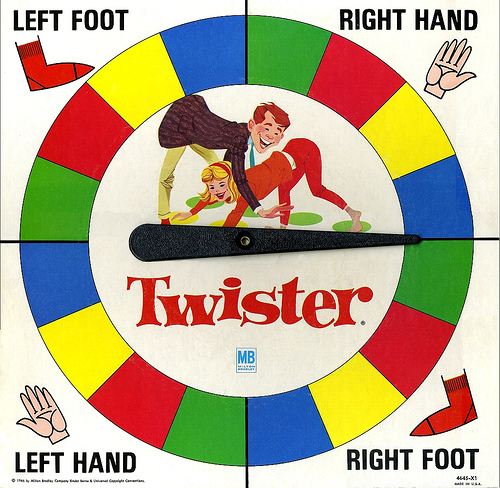
\includegraphics[scale = 0.6]{./images/twister}

\end{frame}
%%%%%%%%%%%%%%%%%%%%%%%%%%%%%%%%%%%%%%%%


\begin{frame}
\frametitle{What is the probability of ``Right Hand Blue?'' \hfill 
\includegraphics[scale = 0.05]{./images/clicker}}
\centering
	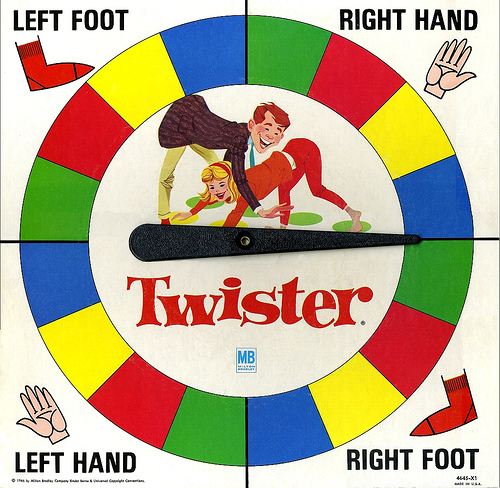
\includegraphics[scale = 0.6]{./images/twister}

\end{frame}
%%%%%%%%%%%%%%%%%%%%%%%%%%%%%%%%%%%%%%%%
\begin{frame}
\frametitle{What is the probability that the spinner lands in any \emph{particular} place?\hfill 
\includegraphics[scale = 0.05]{./images/clicker}}

\begin{center}
	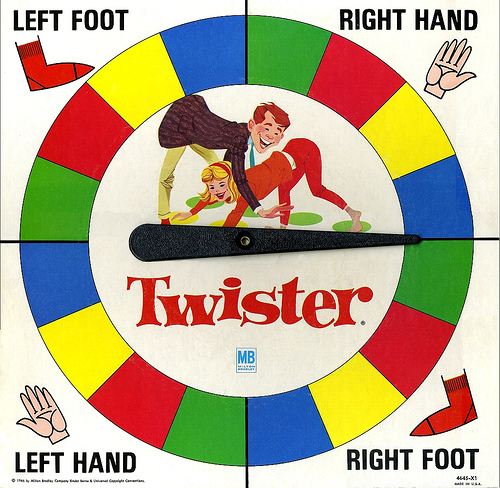
\includegraphics[scale = 0.6]{./images/twister}
\end{center}
\end{frame}




%%%%%%%%%%%%%%%%%%%%%%%%%%%%%%%%%%%%%%%%

\begin{frame}
\frametitle{From Twister to Density -- Probability as \emph{Area}}

\centering
	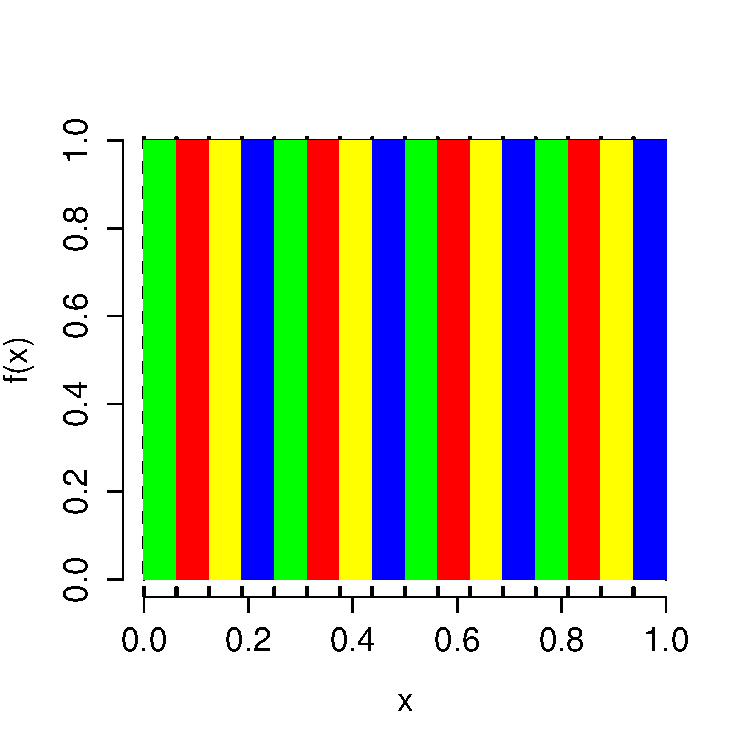
\includegraphics[scale = 0.6]{./images/twister_density}

\end{frame}


%%%%%%%%%%%%%%%%%%%%%%%%%%%%%%%%%%%%%%%%

\begin{frame}
\frametitle{Continuous Random Variables}

For continuous RVs, probability is a matter of finding the area of \emph{intervals}. Individual \emph{points} have \emph{zero} probability.

\end{frame}




%%%%%%%%%%%%%%%%%%%%%%%%%%%%%%%%%%%%%%%%

\begin{frame}
\frametitle{Probability Density Function (PDF)}
For a continuous random variable $X$, 
	$$P(a \leq X \leq b) = \int_a^b f(x) \; dx$$
where $f(x)$ is the \emph{probability density function} for $X$. 
\vspace{2em}

\begin{alertblock}{Extremely Important}
For any realization $x$, $P(X=x) = 0 \neq f(x)$!
\end{alertblock}
\end{frame}
%%%%%%%%%%%%%%%%%%%%%%%%%%%%%%%%%%%%%%%%
\begin{frame}
\frametitle{Properties of PDFs}
\begin{enumerate}
\item $\int_{-\infty}^\infty f(x) \; dx = 1$ 
\item $f(x) \geq 0$ for all $x$
\item $f(x)$ is \emph{not} a probability and can be greater than one!
\item $P(X\leq x_0) = F(x_0) = \int_{-\infty}^{x_0} f(x) \; dx $
\end{enumerate}
\end{frame}
%%%%%%%%%%%%%%%%%%%%%%%%%%%%%%%%%%%%%%%%
\begin{frame}
	\begin{center}
	\huge
		We'll start with the simplest possible example: the Uniform$(0,1)$ RV.
	\end{center} 
\end{frame}


%%%%%%%%%%%%%%%%%%%%%%%%%%%%%%%%%%%%%%%%
\begin{frame}
\frametitle{Uniform$(0,1)$ Random Variable}

\begin{block}{$X \sim \mbox{Uniform}(0,1)$}
We say that $X$ follows a Uniform(0,1) distribution, if it is equally likely to take on \emph{any value} in the range $[0,1]$ and never takes on a value outside this range.
\end{block}

\begin{block}{Uniform PDF}
$f(x) = 1$ for $0\leq x \leq 1$, zero elsewhere.
\end{block}

\end{frame}
%%%%%%%%%%%%%%%%%%%%%%%%%%%%%%%%%%%%%%%%


\begin{frame}
\frametitle{Uniform$(0,1)$ PDF}
\centering
	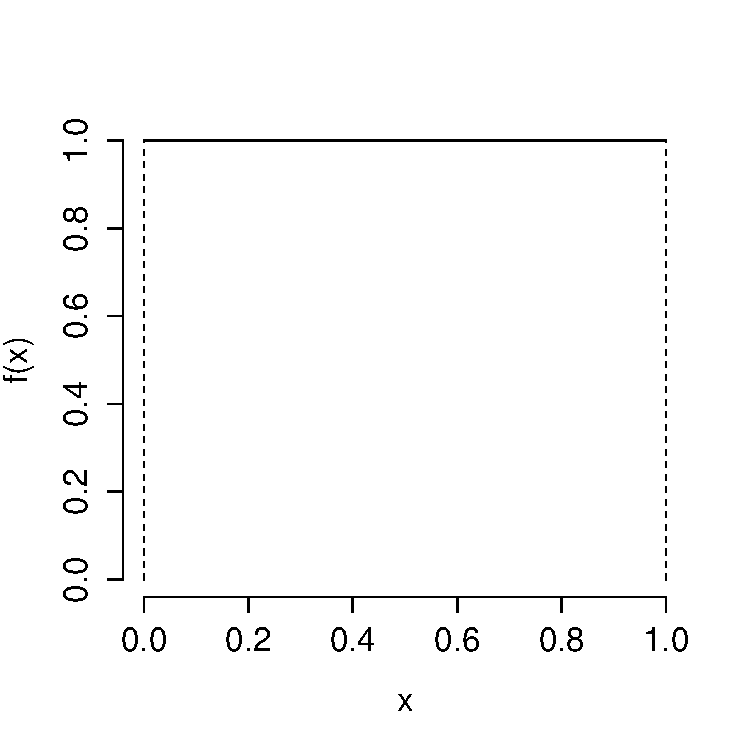
\includegraphics[scale = 0.6]{./images/uniform_density}

\end{frame}


%%%%%%%%%%%%%%%%%%%%%%%%%%%%%%%%%%%%%%%%
\begin{frame}
\frametitle{What is the area of the shaded region? \hfill 
\includegraphics[scale = 0.05]{./images/clicker}}

\centering
	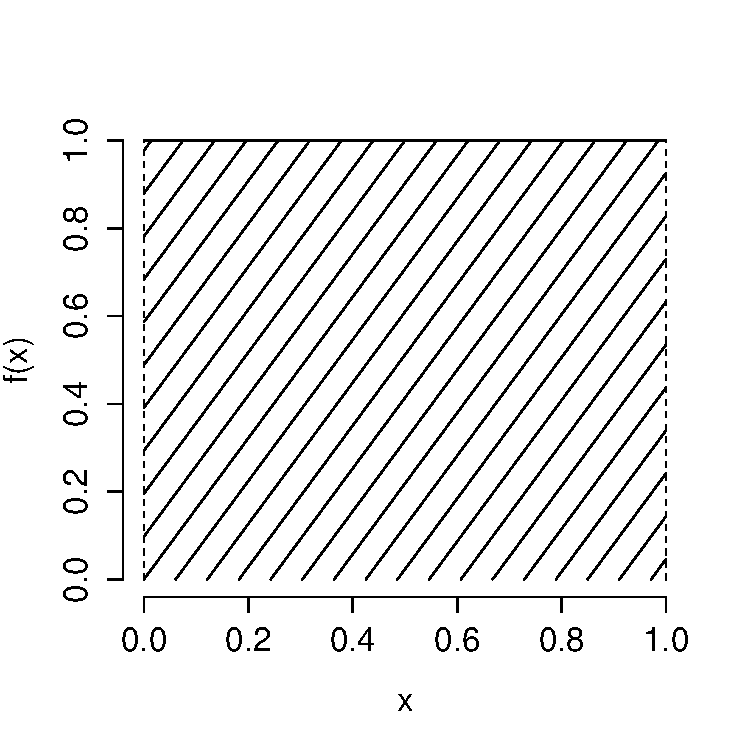
\includegraphics[scale = 0.6]{./images/uniform_density_shaded}

\end{frame}


%%%%%%%%%%%%%%%%%%%%%%%%%%%%%%%%%%%%%%%%

\begin{frame}
\frametitle{What is the area of the shaded region?}

\centering
	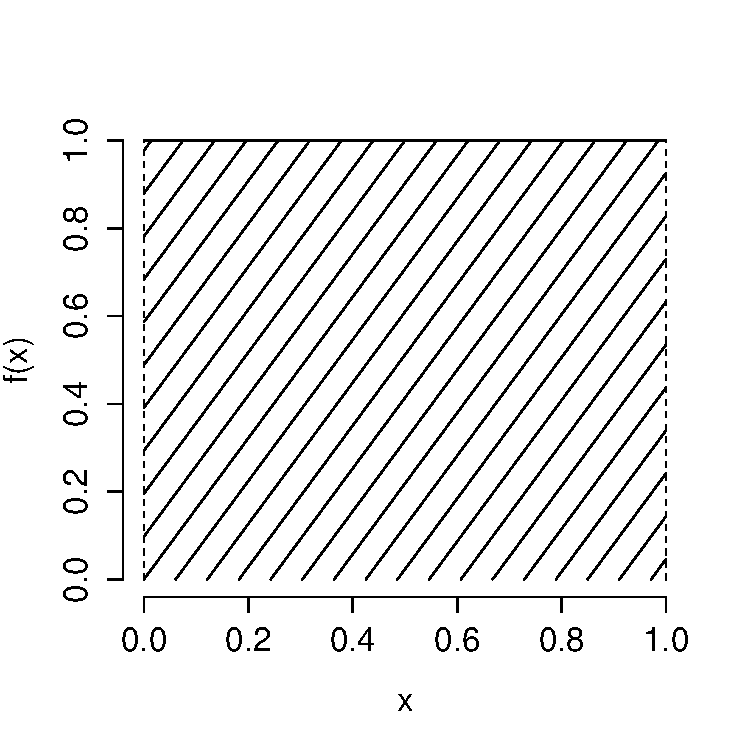
\includegraphics[scale = 0.4]{./images/uniform_density_shaded}
\begin{eqnarray*}
	\int_{-\infty}^{\infty} f(x) \; dx =\pause\int_{0}^1 1 \; dx = \pause \left. x \right|_0^1 =\pause 1 - 0 = 1
\end{eqnarray*}
\end{frame}


%%%%%%%%%%%%%%%%%%%%%%%%%%%%%%%%%%%%%%%%



\begin{frame}
\frametitle{What is the area of the shaded region? \hfill 
\includegraphics[scale = 0.05]{./images/clicker}}
\centering
	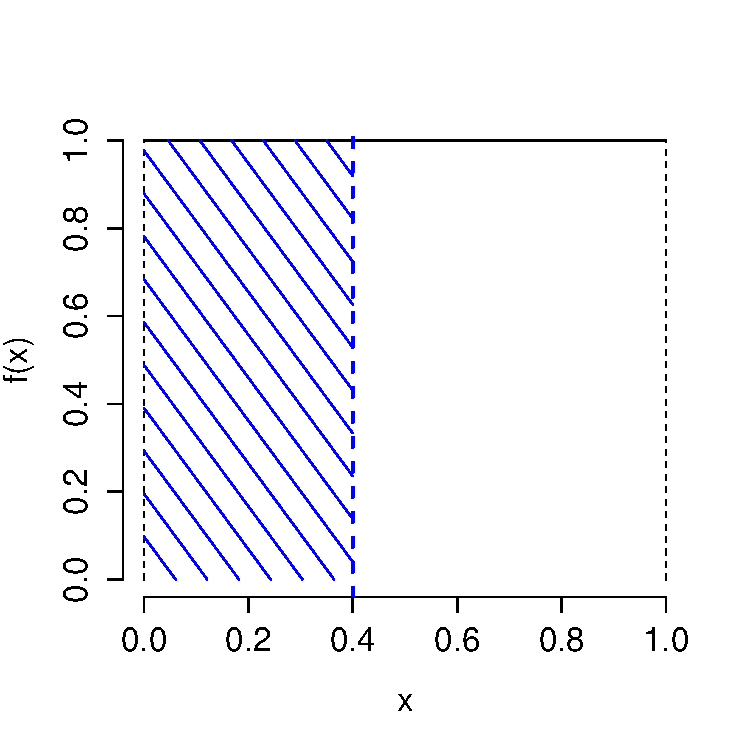
\includegraphics[scale = 0.6]{./images/uniform_density_cdf}

\end{frame}


%%%%%%%%%%%%%%%%%%%%%%%%%%%%%%%%%%%%%%%%

\begin{frame}
\frametitle{$F(0.4) = P(X\leq 0.4) = 0.4$}
\centering
	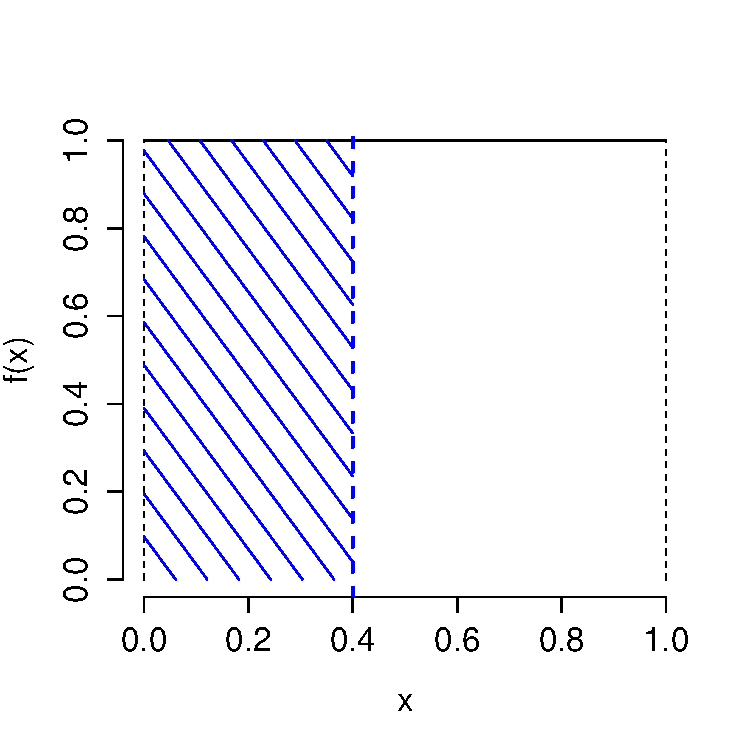
\includegraphics[scale = 0.6]{./images/uniform_density_cdf}

\end{frame}


%%%%%%%%%%%%%%%%%%%%%%%%%%%%%%%%%%%%%%%%


\begin{frame}
\frametitle{Relationship between PDF and CDF}

Integrate the pdf to get the CDF
	$$F(x_0) = P(X\leq x_0) = \int_{-\infty}^{x_0} f(x)\; dx$$
Differentiate the CDF to get the pdf
 	$$f(x) =\frac{d}{dx}F(x)$$
\alert{This is just the Fundamental Theorem of Calculus.}
\end{frame}


%%%%%%%%%%%%%%%%%%%%%%%%%%%%%%%%%%%%%%%%
\begin{frame}
\frametitle{Example: Uniform$(0,1)$ RV}

Integrate the pdf, $f(x) = 1$, to get the CDF
\begin{eqnarray*}
	F(x_0) =\int_{-\infty}^{x_0} f(x)\; dx =\pause \int_{0}^{x_0} 1\; dx = \pause \left. x \right|_0^{x_0} =\pause x_0 - 0 = x_0
\end{eqnarray*}

\vspace{1em}
$$ F(x_0) = \left\{ \begin{array}{c} 0, x_0 < 0\\ x_0, 0\leq x_0 \leq 1\\ 1, x_0 > 1   \end{array}\right.$$
\end{frame}


%%%%%%%%%%%%%%%%%%%%%%%%%%%%%%%%%%%%%%%%
\begin{frame}
\frametitle{Uniform$(0,1)$ CDF}
\centering
	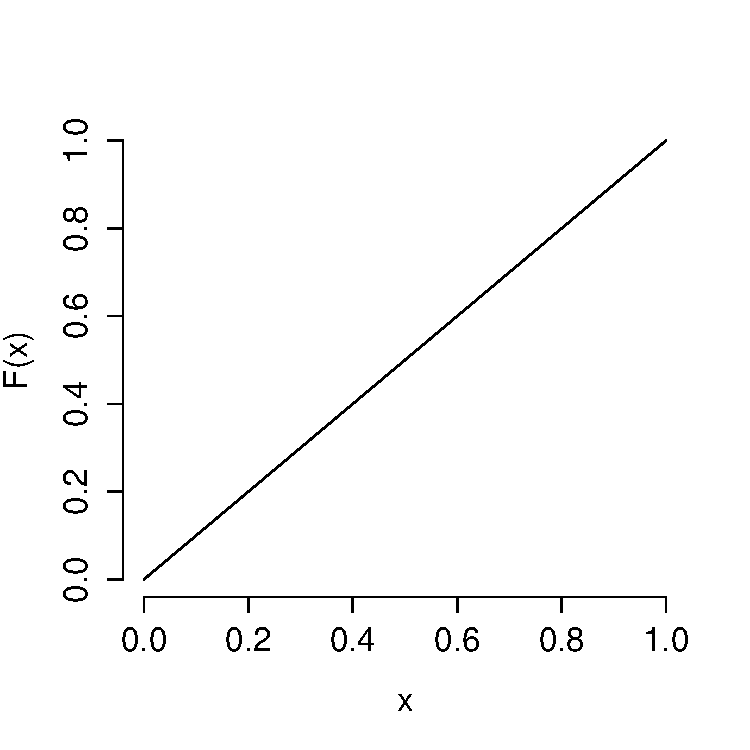
\includegraphics[scale = 0.6]{./images/uniform_CDF}

\end{frame}


%%%%%%%%%%%%%%%%%%%%%%%%%%%%%%%%%%%%%%%%
\begin{frame}
\frametitle{Example: Uniform$(0,1)$ RV}
Differentiate the CDF, $F(x_0) = x_0$, to get the pdf
 \begin{eqnarray*}
	\frac{d}{dx}F(x) =  1 = f(x)
 \end{eqnarray*}
\end{frame}



%%%%%%%%%%%%%%%%%%%%%%%%%%%%%%%%%%%%%%%%


\end{document}
